\documentclass[12pt]{article}
\usepackage[paperwidth=7.44in,paperheight=9.69in,margin=0in,noheadfoot]{geometry}
\usepackage[scale=1.05,osf]{baskervaldx}
\usepackage{tgadventor}
\usepackage[T1]{fontenc}
\usepackage{graphicx,xcolor}
\usepackage[ISBN=978-0-9898975-3-2]{ean13isbn}
\setlength{\parindent}{0pt}
\definecolor{covergreen}{rgb}{0.1,0.5,0.5}
\usepackage{paralist}
\usepackage[letterspace=50]{microtype}
\usepackage{flowfram,ellipsis}
\pagestyle{empty}
\newflowframe{5.5in}{36pt}{.75in}{8.5in}
\newflowframe{2.5in}{36pt}{3.75in}{8in}
\newflowframe{5.5in}{18pt}{.75in}{7.75in}
\newflowframe{2.5in}{1.5in}{.75in}{6.25in}
\newflowframe{5.5in}{.25in}{.75in}{6in}
\newflowframe{4.05in}{2in}{2.15in}{4in}
\newflowframe{5.5in}{1.25in}{.75in}{2.25in}
\newflowframe{2in}{1.1in}{1.6in}{.75in}
\newstaticframe{4in}{36pt}{.5in}{8in}[A]
\newstaticframe{3in}{1.5in}{3.5in}{6.25in}[B]
\newstaticframe{1.5in}{1.5in}{.5in}{4.5in}[C]
%\newstaticframe{1.5in}{1.5in}{5in}{2.75in}[D]
\newstaticframe{1in}{.5in}{3.1in}{3.75in}[E]
\newstaticframe{1in}{1in}{4.5in}{.9in}[F]
\newstaticframe{1in}{1in}{.75in}{.9in}[G]
\begin{document}
\setstaticcontents*{A}{
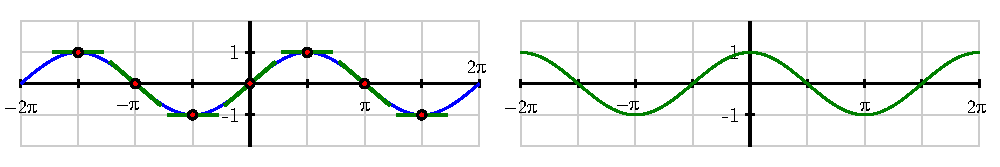
\includegraphics[keepaspectratio,width=4in,height=36pt]{../figures/2_2_sineSoln-eps-converted-to.pdf}
}
\setstaticcontents*{B}{
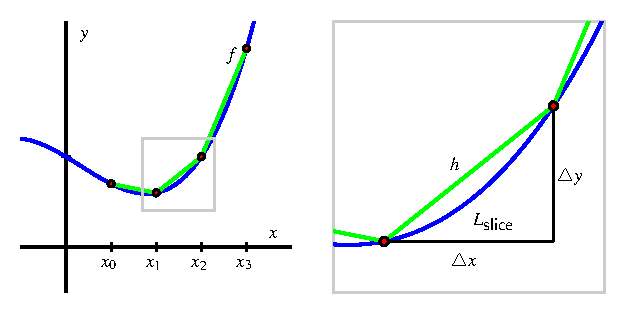
\includegraphics[keepaspectratio,width=3in,height=1.5in]{../figures/6_1_ArcLength-eps-converted-to.pdf}
}
\setstaticcontents*{C}{
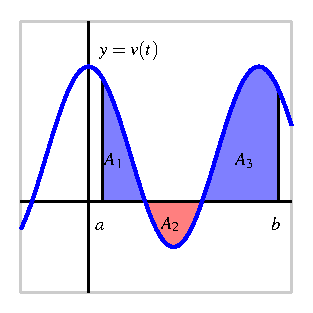
\includegraphics[keepaspectratio,width=1.5in,height=1.5in]{../figures/4_2_Intro-eps-converted-to.pdf}
}
%\setstaticcontents*{D}{
%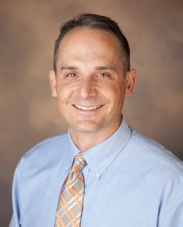
\includegraphics[keepaspectratio,width=1.25in,height=1.25in]{MB.jpg}
%}
\setstaticcontents*{E}{
\includegraphics[keepaspectratio,width=1in,height=.5in]{../figures/CCLicense-eps-converted-to.pdf}
}
\setstaticcontents*{F}{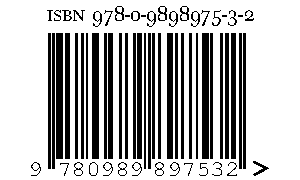
\includegraphics{barcode.pdf}}
\setstaticcontents*{G}{
\includegraphics{qrcode.pdf}}

\fontsize{12pt}{18pt}\selectfont
{\textsf{\textls{\textbf{\color{covergreen}ACTIVE CALCULUS}}}} is different from most existing texts in at least the following ways:
the text is free for download by students and instructors  \framebreak in .pdf format;
in the electronic format, graphics  are in full color \framebreak and there are live 
html links to java applets;
the text  is open  source, \framebreak and   interested instructors
 can gain access to the original source files upon request;
the style of the text requires students to be active learners~\dots~there are very few worked examples in the text, with there
\framebreak  instead being 3--4 activities per section that engage students in
 connecting \framebreak ideas, solving problems, and developing understanding of 
key calculus  ideas;
 each section begins with motivating questions, a brief introduction, 
and a preview activity, all of which are designed to be read and completed
 prior to class;
 the exercises are few in number and challenging in nature.\hfill\framebreak
{\textsf{{\textbf{\color{covergreen}Matthew Boelkins}}}}, {\textsf{{\textbf{\color{covergreen}David Austin}}}}, and {\textsf{{\textbf{\color{covergreen}Steven Schlicker}}}} are professors in the
Department of Mathematics (www.gvsu.edu/math) at Grand Valley State University in Allendale, Michigan.
\hfill 
\framebreak
\begin{flushleft}\qquad
\fontsize{10pt}{12pt}\selectfont
\begin{parbox}{2in}{
Orthogonal Publishing \textsc{l3c} \\
Ann Arbor, Michigan \\
www.orthogonalpublishing.com}
\end{parbox}
\end{flushleft}



\end{document}